\documentclass[twoside]{book}

% Packages required by doxygen
\usepackage{fixltx2e}
\usepackage{calc}
\usepackage{doxygen}
\usepackage[export]{adjustbox} % also loads graphicx
\usepackage{graphicx}
\usepackage[utf8]{inputenc}
\usepackage{makeidx}
\usepackage{multicol}
\usepackage{multirow}
\PassOptionsToPackage{warn}{textcomp}
\usepackage{textcomp}
\usepackage[nointegrals]{wasysym}
\usepackage[table]{xcolor}

% Font selection
\usepackage[T1]{fontenc}
\usepackage[scaled=.90]{helvet}
\usepackage{courier}
\usepackage{amssymb}
\usepackage{sectsty}
\renewcommand{\familydefault}{\sfdefault}
\allsectionsfont{%
  \fontseries{bc}\selectfont%
  \color{darkgray}%
}
\renewcommand{\DoxyLabelFont}{%
  \fontseries{bc}\selectfont%
  \color{darkgray}%
}
\newcommand{\+}{\discretionary{\mbox{\scriptsize$\hookleftarrow$}}{}{}}

% Page & text layout
\usepackage{geometry}
\geometry{%
  a4paper,%
  top=2.5cm,%
  bottom=2.5cm,%
  left=2.5cm,%
  right=2.5cm%
}
\tolerance=750
\hfuzz=15pt
\hbadness=750
\setlength{\emergencystretch}{15pt}
\setlength{\parindent}{0cm}
\setlength{\parskip}{3ex plus 2ex minus 2ex}
\makeatletter
\renewcommand{\paragraph}{%
  \@startsection{paragraph}{4}{0ex}{-1.0ex}{1.0ex}{%
    \normalfont\normalsize\bfseries\SS@parafont%
  }%
}
\renewcommand{\subparagraph}{%
  \@startsection{subparagraph}{5}{0ex}{-1.0ex}{1.0ex}{%
    \normalfont\normalsize\bfseries\SS@subparafont%
  }%
}
\makeatother

% Headers & footers
\usepackage{fancyhdr}
\pagestyle{fancyplain}
\fancyhead[LE]{\fancyplain{}{\bfseries\thepage}}
\fancyhead[CE]{\fancyplain{}{}}
\fancyhead[RE]{\fancyplain{}{\bfseries\leftmark}}
\fancyhead[LO]{\fancyplain{}{\bfseries\rightmark}}
\fancyhead[CO]{\fancyplain{}{}}
\fancyhead[RO]{\fancyplain{}{\bfseries\thepage}}
\fancyfoot[LE]{\fancyplain{}{}}
\fancyfoot[CE]{\fancyplain{}{}}
\fancyfoot[RE]{\fancyplain{}{\bfseries\scriptsize Generated by Doxygen }}
\fancyfoot[LO]{\fancyplain{}{\bfseries\scriptsize Generated by Doxygen }}
\fancyfoot[CO]{\fancyplain{}{}}
\fancyfoot[RO]{\fancyplain{}{}}
\renewcommand{\footrulewidth}{0.4pt}
\renewcommand{\chaptermark}[1]{%
  \markboth{#1}{}%
}
\renewcommand{\sectionmark}[1]{%
  \markright{\thesection\ #1}%
}

% Indices & bibliography
\usepackage{natbib}
\usepackage[titles]{tocloft}
\setcounter{tocdepth}{3}
\setcounter{secnumdepth}{5}
\makeindex

% Hyperlinks (required, but should be loaded last)
\usepackage{ifpdf}
\ifpdf
  \usepackage[pdftex,pagebackref=true]{hyperref}
\else
  \usepackage[ps2pdf,pagebackref=true]{hyperref}
\fi
\hypersetup{%
  colorlinks=true,%
  linkcolor=blue,%
  citecolor=blue,%
  unicode%
}

% Custom commands
\newcommand{\clearemptydoublepage}{%
  \newpage{\pagestyle{empty}\cleardoublepage}%
}

\usepackage{caption}
\captionsetup{labelsep=space,justification=centering,font={bf},singlelinecheck=off,skip=4pt,position=top}

%===== C O N T E N T S =====

\begin{document}

% Titlepage & ToC
\hypersetup{pageanchor=false,
             bookmarksnumbered=true,
             pdfencoding=unicode
            }
\pagenumbering{alph}
\begin{titlepage}
\vspace*{7cm}
\begin{center}%
{\Large Plume }\\
\vspace*{1cm}
{\large Generated by Doxygen 1.8.14}\\
\end{center}
\end{titlepage}
\clearemptydoublepage
\pagenumbering{roman}
\tableofcontents
\clearemptydoublepage
\pagenumbering{arabic}
\hypersetup{pageanchor=true}

%--- Begin generated contents ---
\chapter{Hierarchical Index}
\section{Class Hierarchy}
This inheritance list is sorted roughly, but not completely, alphabetically\+:\begin{DoxyCompactList}
\item Action\+Broadcaster\begin{DoxyCompactList}
\item \contentsline{section}{Plume\+Component}{\pageref{class_plume_component}}{}
\item \contentsline{section}{Plume\+Processor}{\pageref{class_plume_processor}}{}
\end{DoxyCompactList}
\item Action\+Listener\begin{DoxyCompactList}
\item \contentsline{section}{Plume\+Editor}{\pageref{class_plume_editor}}{}
\end{DoxyCompactList}
\item Audio\+Processor\begin{DoxyCompactList}
\item \contentsline{section}{Plume\+Processor}{\pageref{class_plume_processor}}{}
\item \contentsline{section}{Wrapper\+Processor}{\pageref{class_wrapper_processor}}{}
\end{DoxyCompactList}
\item Audio\+Processor\+Editor\begin{DoxyCompactList}
\item \contentsline{section}{Plume\+Editor}{\pageref{class_plume_editor}}{}
\end{DoxyCompactList}
\item Audio\+Processor\+Parameter\begin{DoxyCompactList}
\item \contentsline{section}{Wrapper\+Processor\+:\+:Wrapped\+Parameter}{\pageref{class_wrapper_processor_1_1_wrapped_parameter}}{}
\end{DoxyCompactList}
\item Change\+Broadcaster\begin{DoxyCompactList}
\item \contentsline{section}{Data\+Reader}{\pageref{class_data_reader}}{}
\item \contentsline{section}{Gesture}{\pageref{class_gesture}}{}
\begin{DoxyCompactList}
\item \contentsline{section}{Pitch\+Bend}{\pageref{class_pitch_bend}}{}
\item \contentsline{section}{Roll}{\pageref{class_roll}}{}
\item \contentsline{section}{Tilt}{\pageref{class_tilt}}{}
\item \contentsline{section}{Vibrato}{\pageref{class_vibrato}}{}
\item \contentsline{section}{Wave}{\pageref{class_wave}}{}
\end{DoxyCompactList}
\item \contentsline{section}{Gesture\+Array}{\pageref{class_gesture_array}}{}
\item \contentsline{section}{Mapper\+Component}{\pageref{class_mapper_component}}{}
\item \contentsline{section}{Plugin\+Wrapper}{\pageref{class_plugin_wrapper}}{}
\end{DoxyCompactList}
\item Change\+Listener\begin{DoxyCompactList}
\item \contentsline{section}{Gesture\+Array}{\pageref{class_gesture_array}}{}
\item \contentsline{section}{Mapper\+Component}{\pageref{class_mapper_component}}{}
\end{DoxyCompactList}
\item Component\begin{DoxyCompactList}
\item \contentsline{section}{Gesture\+Panel}{\pageref{class_gesture_panel}}{}
\item \contentsline{section}{Gesture\+Panel\+:\+:Gesture\+Component}{\pageref{class_gesture_panel_1_1_gesture_component}}{}
\item \contentsline{section}{Header\+Component}{\pageref{class_header_component}}{}
\item \contentsline{section}{Mapped\+Parameter\+Component}{\pageref{class_mapped_parameter_component}}{}
\item \contentsline{section}{Mapper\+Component}{\pageref{class_mapper_component}}{}
\item \contentsline{section}{Midi\+Mode\+Component}{\pageref{class_midi_mode_component}}{}
\item \contentsline{section}{Moving\+Cursor}{\pageref{class_moving_cursor}}{}
\item \contentsline{section}{Plume\+Component}{\pageref{class_plume_component}}{}
\item \contentsline{section}{Preset\+Component}{\pageref{class_preset_component}}{}
\item \contentsline{section}{Side\+Bar\+Component}{\pageref{class_side_bar_component}}{}
\item \contentsline{section}{Tuner}{\pageref{class_tuner}}{}
\begin{DoxyCompactList}
\item \contentsline{section}{One\+Range\+Tuner}{\pageref{class_one_range_tuner}}{}
\begin{DoxyCompactList}
\item \contentsline{section}{Roll\+Tuner}{\pageref{class_roll_tuner}}{}
\item \contentsline{section}{Tilt\+Tuner}{\pageref{class_tilt_tuner}}{}
\end{DoxyCompactList}
\item \contentsline{section}{Symmetrical\+Tuner}{\pageref{class_symmetrical_tuner}}{}
\begin{DoxyCompactList}
\item \contentsline{section}{Vibrato\+Tuner}{\pageref{class_vibrato_tuner}}{}
\end{DoxyCompactList}
\item \contentsline{section}{Two\+Range\+Tuner}{\pageref{class_two_range_tuner}}{}
\begin{DoxyCompactList}
\item \contentsline{section}{Pitch\+Bend\+Tuner}{\pageref{class_pitch_bend_tuner}}{}
\end{DoxyCompactList}
\end{DoxyCompactList}
\item \contentsline{section}{Wrapper\+Component}{\pageref{class_wrapper_component}}{}
\end{DoxyCompactList}
\item Document\+Window\begin{DoxyCompactList}
\item \contentsline{section}{Wrapper\+Editor\+Window}{\pageref{class_wrapper_editor_window}}{}
\end{DoxyCompactList}
\item Interprocess\+Connection\begin{DoxyCompactList}
\item \contentsline{section}{Data\+Reader}{\pageref{class_data_reader}}{}
\end{DoxyCompactList}
\item List\+Box\begin{DoxyCompactList}
\item \contentsline{section}{Preset\+Box}{\pageref{class_preset_box}}{}
\end{DoxyCompactList}
\item List\+Box\+Model\begin{DoxyCompactList}
\item \contentsline{section}{Preset\+Box}{\pageref{class_preset_box}}{}
\end{DoxyCompactList}
\item Listener\begin{DoxyCompactList}
\item \contentsline{section}{Gesture\+Panel\+:\+:Gesture\+Component}{\pageref{class_gesture_panel_1_1_gesture_component}}{}
\item \contentsline{section}{Header\+Component}{\pageref{class_header_component}}{}
\item \contentsline{section}{Mapped\+Parameter\+Component}{\pageref{class_mapped_parameter_component}}{}
\item \contentsline{section}{Mapper\+Component}{\pageref{class_mapper_component}}{}
\item \contentsline{section}{Plume\+Editor}{\pageref{class_plume_editor}}{}
\item \contentsline{section}{Preset\+Component}{\pageref{class_preset_component}}{}
\item \contentsline{section}{Side\+Bar\+Component}{\pageref{class_side_bar_component}}{}
\item \contentsline{section}{Wrapper\+Component}{\pageref{class_wrapper_component}}{}
\end{DoxyCompactList}
\item Listener\begin{DoxyCompactList}
\item \contentsline{section}{One\+Range\+Tuner}{\pageref{class_one_range_tuner}}{}
\item \contentsline{section}{Symmetrical\+Tuner}{\pageref{class_symmetrical_tuner}}{}
\item \contentsline{section}{Two\+Range\+Tuner}{\pageref{class_two_range_tuner}}{}
\end{DoxyCompactList}
\item Listener\begin{DoxyCompactList}
\item \contentsline{section}{Midi\+Mode\+Component}{\pageref{class_midi_mode_component}}{}
\end{DoxyCompactList}
\item Listener\begin{DoxyCompactList}
\item \contentsline{section}{Mapped\+Parameter\+Component}{\pageref{class_mapped_parameter_component}}{}
\item \contentsline{section}{Mapper\+Component}{\pageref{class_mapper_component}}{}
\item \contentsline{section}{Midi\+Mode\+Component}{\pageref{class_midi_mode_component}}{}
\item \contentsline{section}{One\+Range\+Tuner}{\pageref{class_one_range_tuner}}{}
\item \contentsline{section}{Preset\+Box}{\pageref{class_preset_box}}{}
\item \contentsline{section}{Symmetrical\+Tuner}{\pageref{class_symmetrical_tuner}}{}
\item \contentsline{section}{Two\+Range\+Tuner}{\pageref{class_two_range_tuner}}{}
\end{DoxyCompactList}
\item Listener\begin{DoxyCompactList}
\item \contentsline{section}{Plugin\+Wrapper}{\pageref{class_plugin_wrapper}}{}
\end{DoxyCompactList}
\item Listener\begin{DoxyCompactList}
\item \contentsline{section}{Gesture\+Panel}{\pageref{class_gesture_panel}}{}
\end{DoxyCompactList}
\item Look\+And\+Feel\+\_\+\+V4\begin{DoxyCompactList}
\item \contentsline{section}{P\+L\+U\+ME\+:\+:Plume\+Look\+And\+Feel}{\pageref{class_p_l_u_m_e_1_1_plume_look_and_feel}}{}
\begin{DoxyCompactList}
\item \contentsline{section}{P\+L\+U\+ME\+:\+:One\+Range\+Tuner\+Look\+And\+Feel}{\pageref{class_p_l_u_m_e_1_1_one_range_tuner_look_and_feel}}{}
\item \contentsline{section}{P\+L\+U\+ME\+:\+:Two\+Range\+Tuner\+Look\+And\+Feel}{\pageref{class_p_l_u_m_e_1_1_two_range_tuner_look_and_feel}}{}
\end{DoxyCompactList}
\end{DoxyCompactList}
\item \contentsline{section}{Gesture\+:\+:Mapped\+Parameter}{\pageref{struct_gesture_1_1_mapped_parameter}}{}
\item \contentsline{section}{P\+L\+U\+ME\+:\+:colour\+:\+:Plume\+Theme}{\pageref{class_p_l_u_m_e_1_1colour_1_1_plume_theme}}{}
\item \contentsline{section}{Preset\+Handler}{\pageref{class_preset_handler}}{}
\item Timer\begin{DoxyCompactList}
\item \contentsline{section}{Gesture\+Panel}{\pageref{class_gesture_panel}}{}
\end{DoxyCompactList}
\end{DoxyCompactList}

\chapter{Class Index}
\section{Class List}
Here are the classes, structs, unions and interfaces with brief descriptions\+:\begin{DoxyCompactList}
\item\contentsline{section}{\mbox{\hyperlink{class_data_reader}{Data\+Reader}} \\*Class that gets the raw data from the ring }{\pageref{class_data_reader}}{}
\item\contentsline{section}{\mbox{\hyperlink{class_gesture}{Gesture}} \\*\mbox{\hyperlink{class_gesture}{Gesture}} base class }{\pageref{class_gesture}}{}
\item\contentsline{section}{\mbox{\hyperlink{class_gesture_array}{Gesture\+Array}} \\*Class that holds an array of \mbox{\hyperlink{class_gesture}{Gesture}}, with several methods to use them }{\pageref{class_gesture_array}}{}
\item\contentsline{section}{\mbox{\hyperlink{class_gesture_panel_1_1_gesture_component}{Gesture\+Panel\+::\+Gesture\+Component}} }{\pageref{class_gesture_panel_1_1_gesture_component}}{}
\item\contentsline{section}{\mbox{\hyperlink{class_gesture_panel}{Gesture\+Panel}} }{\pageref{class_gesture_panel}}{}
\item\contentsline{section}{\mbox{\hyperlink{class_header_component}{Header\+Component}} }{\pageref{class_header_component}}{}
\item\contentsline{section}{\mbox{\hyperlink{struct_gesture_1_1_mapped_parameter}{Gesture\+::\+Mapped\+Parameter}} \\*Struct that holds a reference to an Audio\+Processor\+Parameter from the wrapped plugin and a range }{\pageref{struct_gesture_1_1_mapped_parameter}}{}
\item\contentsline{section}{\mbox{\hyperlink{class_mapped_parameter_component}{Mapped\+Parameter\+Component}} }{\pageref{class_mapped_parameter_component}}{}
\item\contentsline{section}{\mbox{\hyperlink{class_mapper_component}{Mapper\+Component}} }{\pageref{class_mapper_component}}{}
\item\contentsline{section}{\mbox{\hyperlink{class_midi_mode_component}{Midi\+Mode\+Component}} }{\pageref{class_midi_mode_component}}{}
\item\contentsline{section}{\mbox{\hyperlink{class_moving_cursor}{Moving\+Cursor}} }{\pageref{class_moving_cursor}}{}
\item\contentsline{section}{\mbox{\hyperlink{class_one_range_tuner}{One\+Range\+Tuner}} }{\pageref{class_one_range_tuner}}{}
\item\contentsline{section}{\mbox{\hyperlink{class_one_range_tuner_look_and_feel}{One\+Range\+Tuner\+Look\+And\+Feel}} }{\pageref{class_one_range_tuner_look_and_feel}}{}
\item\contentsline{section}{\mbox{\hyperlink{class_pitch_bend}{Pitch\+Bend}} \\*\mbox{\hyperlink{class_pitch_bend}{Pitch\+Bend}} gesture class }{\pageref{class_pitch_bend}}{}
\item\contentsline{section}{\mbox{\hyperlink{class_pitch_bend_tuner}{Pitch\+Bend\+Tuner}} }{\pageref{class_pitch_bend_tuner}}{}
\item\contentsline{section}{\mbox{\hyperlink{class_plugin_wrapper}{Plugin\+Wrapper}} \\*Class that manages the plugin wrapping function of plume }{\pageref{class_plugin_wrapper}}{}
\item\contentsline{section}{\mbox{\hyperlink{class_plume_editor}{Plume\+Editor}} \\*Plume\textquotesingle{}s editor component. Holds the ui of the plugin }{\pageref{class_plume_editor}}{}
\item\contentsline{section}{\mbox{\hyperlink{class_plume_look_and_feel}{Plume\+Look\+And\+Feel}} }{\pageref{class_plume_look_and_feel}}{}
\item\contentsline{section}{\mbox{\hyperlink{class_plume_processor}{Plume\+Processor}} \\*Plume\textquotesingle{}s processor object }{\pageref{class_plume_processor}}{}
\item\contentsline{section}{\mbox{\hyperlink{class_preset_component}{Preset\+Component}} }{\pageref{class_preset_component}}{}
\item\contentsline{section}{\mbox{\hyperlink{class_roll}{Roll}} \\*\mbox{\hyperlink{class_roll}{Roll}} gesture class }{\pageref{class_roll}}{}
\item\contentsline{section}{\mbox{\hyperlink{class_roll_tuner}{Roll\+Tuner}} }{\pageref{class_roll_tuner}}{}
\item\contentsline{section}{\mbox{\hyperlink{class_side_bar_component}{Side\+Bar\+Component}} }{\pageref{class_side_bar_component}}{}
\item\contentsline{section}{\mbox{\hyperlink{class_symmetrical_tuner}{Symmetrical\+Tuner}} }{\pageref{class_symmetrical_tuner}}{}
\item\contentsline{section}{\mbox{\hyperlink{class_tilt}{Tilt}} \\*\mbox{\hyperlink{class_tilt}{Tilt}} gesture class }{\pageref{class_tilt}}{}
\item\contentsline{section}{\mbox{\hyperlink{class_tilt_tuner}{Tilt\+Tuner}} }{\pageref{class_tilt_tuner}}{}
\item\contentsline{section}{\mbox{\hyperlink{class_tuner}{Tuner}} }{\pageref{class_tuner}}{}
\item\contentsline{section}{\mbox{\hyperlink{class_two_range_tuner}{Two\+Range\+Tuner}} }{\pageref{class_two_range_tuner}}{}
\item\contentsline{section}{\mbox{\hyperlink{class_two_range_tuner_look_and_feel}{Two\+Range\+Tuner\+Look\+And\+Feel}} }{\pageref{class_two_range_tuner_look_and_feel}}{}
\item\contentsline{section}{\mbox{\hyperlink{class_vibrato}{Vibrato}} \\*\mbox{\hyperlink{class_vibrato}{Vibrato}} gesture class }{\pageref{class_vibrato}}{}
\item\contentsline{section}{\mbox{\hyperlink{class_vibrato_tuner}{Vibrato\+Tuner}} }{\pageref{class_vibrato_tuner}}{}
\item\contentsline{section}{\mbox{\hyperlink{class_wave}{Wave}} }{\pageref{class_wave}}{}
\item\contentsline{section}{\mbox{\hyperlink{class_wrapper_processor_1_1_wrapped_parameter}{Wrapper\+Processor\+::\+Wrapped\+Parameter}} }{\pageref{class_wrapper_processor_1_1_wrapped_parameter}}{}
\item\contentsline{section}{\mbox{\hyperlink{class_wrapper_component}{Wrapper\+Component}} }{\pageref{class_wrapper_component}}{}
\item\contentsline{section}{\mbox{\hyperlink{class_wrapper_editor_window}{Wrapper\+Editor\+Window}} \\*A desktop window containing the wrapped plugin\textquotesingle{}s G\+UI }{\pageref{class_wrapper_editor_window}}{}
\item\contentsline{section}{\mbox{\hyperlink{class_wrapper_processor}{Wrapper\+Processor}} }{\pageref{class_wrapper_processor}}{}
\end{DoxyCompactList}

\chapter{Class Documentation}
\input{class_data_reader}
\input{class_gesture}
\input{class_gesture_array}
\input{class_gesture_panel_1_1_gesture_component}
\input{class_gesture_panel}
\input{class_pitch_bend}
\input{class_plugin_wrapper}
\hypertarget{class_plume_editor}{}\section{Plume\+Editor Class Reference}
\label{class_plume_editor}\index{Plume\+Editor@{Plume\+Editor}}


Plume\textquotesingle{}s editor component. Holds the ui of the plugin.  




{\ttfamily \#include $<$Plugin\+Editor.\+h$>$}

Inheritance diagram for Plume\+Editor\+:\begin{figure}[H]
\begin{center}
\leavevmode
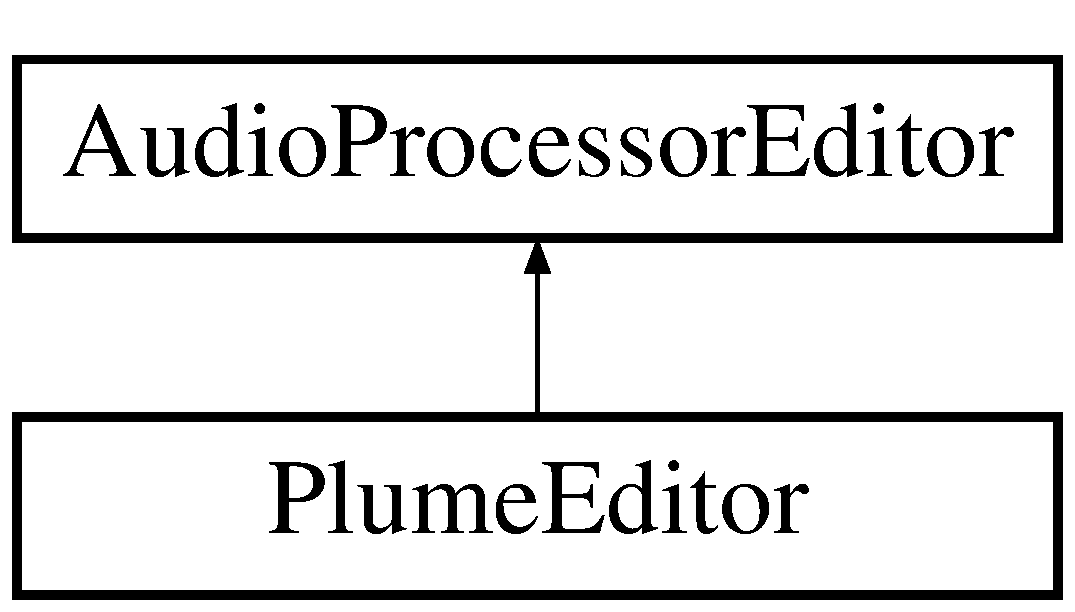
\includegraphics[height=2.000000cm]{class_plume_editor}
\end{center}
\end{figure}
\subsection*{Public Member Functions}
\begin{DoxyCompactItemize}
\item 
\mbox{\hyperlink{class_plume_editor_a0b9b4a952769836ca43c49ed020951f9}{Plume\+Editor}} (\mbox{\hyperlink{class_plume_processor}{Plume\+Processor}} \&p)
\begin{DoxyCompactList}\small\item\em Constructor. \end{DoxyCompactList}\item 
\mbox{\Hypertarget{class_plume_editor_af16dd852a3419961627d070d62e3e644}\label{class_plume_editor_af16dd852a3419961627d070d62e3e644}} 
\mbox{\hyperlink{class_plume_editor_af16dd852a3419961627d070d62e3e644}{$\sim$\+Plume\+Editor}} ()
\begin{DoxyCompactList}\small\item\em Destructor. \end{DoxyCompactList}\item 
\mbox{\Hypertarget{class_plume_editor_a3b31e2023faf921f446b132b24a917c0}\label{class_plume_editor_a3b31e2023faf921f446b132b24a917c0}} 
void \mbox{\hyperlink{class_plume_editor_a3b31e2023faf921f446b132b24a917c0}{paint}} (Graphics \&g) override
\begin{DoxyCompactList}\small\item\em J\+U\+CE Components\textquotesingle{} paint method. \end{DoxyCompactList}\item 
\mbox{\Hypertarget{class_plume_editor_aa42064f898f3a543173c5b29c7b2932c}\label{class_plume_editor_aa42064f898f3a543173c5b29c7b2932c}} 
void \mbox{\hyperlink{class_plume_editor_aa42064f898f3a543173c5b29c7b2932c}{resized}} () override
\begin{DoxyCompactList}\small\item\em J\+U\+CE Components\textquotesingle{} resized method. \end{DoxyCompactList}\item 
void \mbox{\hyperlink{class_plume_editor_a5d593b33e5e4e33827928dbcdc272416}{change\+Listener\+Callback}} (Change\+Broadcaster $\ast$source) override
\begin{DoxyCompactList}\small\item\em Callback to a change message sent by the processor. \end{DoxyCompactList}\item 
void \mbox{\hyperlink{class_plume_editor_acddc96d095aeb53f7a4ee6cf1f3265e6}{update\+Full\+Interface}} ()
\begin{DoxyCompactList}\small\item\em Method that sets a full interface update. \end{DoxyCompactList}\end{DoxyCompactItemize}


\subsection{Detailed Description}
Plume\textquotesingle{}s editor component. Holds the ui of the plugin. 

Holds plumes G\+UI. This component will create the child components that will handle the 3 interface blocks\+: wrapper, presets, and gestures. 

\subsection{Constructor \& Destructor Documentation}
\mbox{\Hypertarget{class_plume_editor_a0b9b4a952769836ca43c49ed020951f9}\label{class_plume_editor_a0b9b4a952769836ca43c49ed020951f9}} 
\index{Plume\+Editor@{Plume\+Editor}!Plume\+Editor@{Plume\+Editor}}
\index{Plume\+Editor@{Plume\+Editor}!Plume\+Editor@{Plume\+Editor}}
\subsubsection{\texorpdfstring{Plume\+Editor()}{PlumeEditor()}}
{\footnotesize\ttfamily Plume\+Editor\+::\+Plume\+Editor (\begin{DoxyParamCaption}\item[{\mbox{\hyperlink{class_plume_processor}{Plume\+Processor}} \&}]{p }\end{DoxyParamCaption})}



Constructor. 

Draws the background, calls the subcomponents and sets their bounds accordingly.


\begin{DoxyParams}{Parameters}
{\em p} & Reference to Plume\textquotesingle{}s processor object. \\
\hline
\end{DoxyParams}


\subsection{Member Function Documentation}
\mbox{\Hypertarget{class_plume_editor_a5d593b33e5e4e33827928dbcdc272416}\label{class_plume_editor_a5d593b33e5e4e33827928dbcdc272416}} 
\index{Plume\+Editor@{Plume\+Editor}!change\+Listener\+Callback@{change\+Listener\+Callback}}
\index{change\+Listener\+Callback@{change\+Listener\+Callback}!Plume\+Editor@{Plume\+Editor}}
\subsubsection{\texorpdfstring{change\+Listener\+Callback()}{changeListenerCallback()}}
{\footnotesize\ttfamily void Plume\+Editor\+::change\+Listener\+Callback (\begin{DoxyParamCaption}\item[{Change\+Broadcaster $\ast$}]{source }\end{DoxyParamCaption})\hspace{0.3cm}{\ttfamily [override]}}



Callback to a change message sent by the processor. 

This method is called by the processor when it needs the interface to be fully updated. It calls the method update\+Full\+Interface. sets the right current wrapped plugin, preset and gestures. \mbox{\Hypertarget{class_plume_editor_acddc96d095aeb53f7a4ee6cf1f3265e6}\label{class_plume_editor_acddc96d095aeb53f7a4ee6cf1f3265e6}} 
\index{Plume\+Editor@{Plume\+Editor}!update\+Full\+Interface@{update\+Full\+Interface}}
\index{update\+Full\+Interface@{update\+Full\+Interface}!Plume\+Editor@{Plume\+Editor}}
\subsubsection{\texorpdfstring{update\+Full\+Interface()}{updateFullInterface()}}
{\footnotesize\ttfamily void Plume\+Editor\+::update\+Full\+Interface (\begin{DoxyParamCaption}{ }\end{DoxyParamCaption})}



Method that sets a full interface update. 

This method is called after a change message is sent by the processor. It sets the right current wrapped plugin, preset and gestures. 

The documentation for this class was generated from the following files\+:\begin{DoxyCompactItemize}
\item 
D\+:/\+Workspace/\+Git\+Workspace/\+Plume/\+Plume/\+Source/\+Plugin/Plugin\+Editor.\+h\item 
D\+:/\+Workspace/\+Git\+Workspace/\+Plume/\+Plume/\+Source/\+Plugin/Plugin\+Editor.\+cpp\end{DoxyCompactItemize}

\input{class_plume_look_and_feel}
\hypertarget{class_plume_processor}{}\section{Plume\+Processor Class Reference}
\label{class_plume_processor}\index{Plume\+Processor@{Plume\+Processor}}


Plume\textquotesingle{}s processor object.  




{\ttfamily \#include $<$Plugin\+Processor.\+h$>$}

Inheritance diagram for Plume\+Processor\+:\begin{figure}[H]
\begin{center}
\leavevmode
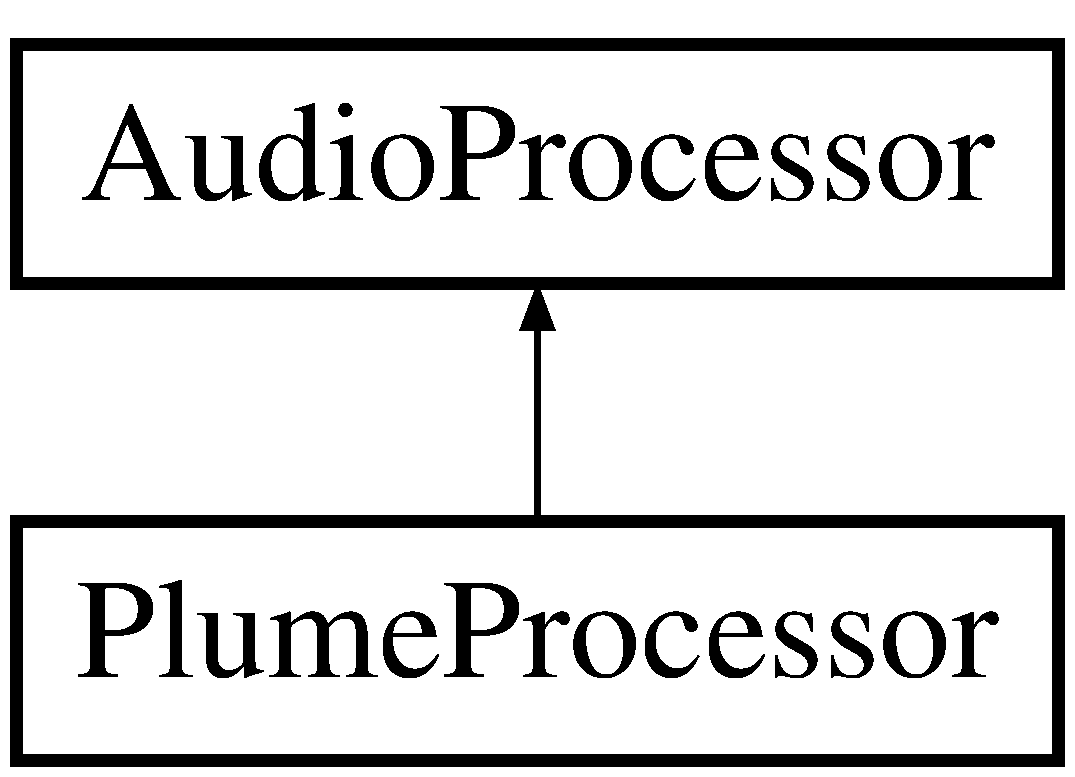
\includegraphics[height=2.000000cm]{class_plume_processor}
\end{center}
\end{figure}
\subsection*{Public Member Functions}
\begin{DoxyCompactItemize}
\item 
\mbox{\hyperlink{class_plume_processor_a1462b7f98f4677da0dab2d98dd8da1e1}{Plume\+Processor}} ()
\begin{DoxyCompactList}\small\item\em Constructor. \end{DoxyCompactList}\item 
\mbox{\Hypertarget{class_plume_processor_a3ff1acd929c81502079017721525a2df}\label{class_plume_processor_a3ff1acd929c81502079017721525a2df}} 
\mbox{\hyperlink{class_plume_processor_a3ff1acd929c81502079017721525a2df}{$\sim$\+Plume\+Processor}} ()
\begin{DoxyCompactList}\small\item\em Destructor. \end{DoxyCompactList}\item 
\mbox{\Hypertarget{class_plume_processor_a86a4085b844401c13d952e3936605b78}\label{class_plume_processor_a86a4085b844401c13d952e3936605b78}} 
void {\bfseries prepare\+To\+Play} (double sample\+Rate, int samples\+Per\+Block) override
\item 
\mbox{\Hypertarget{class_plume_processor_ac85f0efc3d2dcd25d805c3d096c5fad8}\label{class_plume_processor_ac85f0efc3d2dcd25d805c3d096c5fad8}} 
void {\bfseries release\+Resources} () override
\item 
\mbox{\Hypertarget{class_plume_processor_a8f659b42f6d4f2fe00c9feec53f9f5b7}\label{class_plume_processor_a8f659b42f6d4f2fe00c9feec53f9f5b7}} 
bool {\bfseries is\+Buses\+Layout\+Supported} (const Buses\+Layout \&layouts) const override
\item 
\mbox{\Hypertarget{class_plume_processor_aa47e4738eae67255b42533566bca5f6b}\label{class_plume_processor_aa47e4738eae67255b42533566bca5f6b}} 
void {\bfseries process\+Block} (Audio\+Buffer$<$ float $>$ \&, Midi\+Buffer \&) override
\item 
\mbox{\Hypertarget{class_plume_processor_ad8a4c43c38f0be73c8c5845a3d42a011}\label{class_plume_processor_ad8a4c43c38f0be73c8c5845a3d42a011}} 
Audio\+Processor\+Editor $\ast$ {\bfseries create\+Editor} () override
\item 
\mbox{\Hypertarget{class_plume_processor_acd298ef63a793a2a713048a758d6aa7c}\label{class_plume_processor_acd298ef63a793a2a713048a758d6aa7c}} 
bool {\bfseries has\+Editor} () const override
\item 
\mbox{\Hypertarget{class_plume_processor_ae94a4572fc37682092a145a62606b0bb}\label{class_plume_processor_ae94a4572fc37682092a145a62606b0bb}} 
const String {\bfseries get\+Name} () const override
\item 
\mbox{\Hypertarget{class_plume_processor_a9dfd593b13b864f6d646600453b983bc}\label{class_plume_processor_a9dfd593b13b864f6d646600453b983bc}} 
bool {\bfseries accepts\+Midi} () const override
\item 
\mbox{\Hypertarget{class_plume_processor_af53ebafbc9dbb53b5f417f06814e5753}\label{class_plume_processor_af53ebafbc9dbb53b5f417f06814e5753}} 
bool {\bfseries produces\+Midi} () const override
\item 
\mbox{\Hypertarget{class_plume_processor_a92025e451d25175363b38f5fa1f99e8a}\label{class_plume_processor_a92025e451d25175363b38f5fa1f99e8a}} 
bool {\bfseries is\+Midi\+Effect} () const override
\item 
\mbox{\Hypertarget{class_plume_processor_ae85b56bdc30fc398bdc3e6a9b40c733a}\label{class_plume_processor_ae85b56bdc30fc398bdc3e6a9b40c733a}} 
double {\bfseries get\+Tail\+Length\+Seconds} () const override
\item 
\mbox{\Hypertarget{class_plume_processor_acc125f472abf81a2273f7aafe75302ec}\label{class_plume_processor_acc125f472abf81a2273f7aafe75302ec}} 
int {\bfseries get\+Num\+Programs} () override
\item 
\mbox{\Hypertarget{class_plume_processor_a5bf89a890c12f02dd352a523c1a88f64}\label{class_plume_processor_a5bf89a890c12f02dd352a523c1a88f64}} 
int {\bfseries get\+Current\+Program} () override
\item 
\mbox{\Hypertarget{class_plume_processor_a909a5331670eb7b2e722498e755bf890}\label{class_plume_processor_a909a5331670eb7b2e722498e755bf890}} 
void {\bfseries set\+Current\+Program} (int index) override
\item 
\mbox{\Hypertarget{class_plume_processor_ac16c6d0751467defa92a523ffb6af939}\label{class_plume_processor_ac16c6d0751467defa92a523ffb6af939}} 
const String {\bfseries get\+Program\+Name} (int index) override
\item 
\mbox{\Hypertarget{class_plume_processor_a28ce5f77d4e4871ff57ade3e730b5cd9}\label{class_plume_processor_a28ce5f77d4e4871ff57ade3e730b5cd9}} 
void {\bfseries change\+Program\+Name} (int index, const String \&new\+Name) override
\item 
void \mbox{\hyperlink{class_plume_processor_ae06dd312c3dc3ba7389ce44fd74cbc18}{get\+State\+Information}} (Memory\+Block \&dest\+Data) override
\begin{DoxyCompactList}\small\item\em State save method. \end{DoxyCompactList}\item 
void \mbox{\hyperlink{class_plume_processor_aa7ab9da73c37f6db69ea6c7e1e4a0211}{set\+State\+Information}} (const void $\ast$data, int size\+In\+Bytes) override
\begin{DoxyCompactList}\small\item\em State load method. \end{DoxyCompactList}\item 
\mbox{\Hypertarget{class_plume_processor_ad29b07ddcd526e44529e361374c8c99e}\label{class_plume_processor_ad29b07ddcd526e44529e361374c8c99e}} 
void {\bfseries create\+Plugin\+Xml} (Xml\+Element \&wrapper\+Data)
\item 
\mbox{\Hypertarget{class_plume_processor_a14455799e2ddefd50b860d4492845509}\label{class_plume_processor_a14455799e2ddefd50b860d4492845509}} 
void {\bfseries create\+Gesture\+Xml} (Xml\+Element \&wrapper\+Data)
\item 
\mbox{\Hypertarget{class_plume_processor_a08587fb2663557a8250132502785205c}\label{class_plume_processor_a08587fb2663557a8250132502785205c}} 
void {\bfseries load\+Plugin\+Xml} (const Xml\+Element \&plugin\+Data)
\item 
\mbox{\Hypertarget{class_plume_processor_a988e2a3ce47486bd8dfc5d5702420a7e}\label{class_plume_processor_a988e2a3ce47486bd8dfc5d5702420a7e}} 
void {\bfseries load\+Gesture\+Xml} (const Xml\+Element \&gesture\+Data)
\item 
\mbox{\hyperlink{class_plugin_wrapper}{Plugin\+Wrapper}} \& \mbox{\hyperlink{class_plume_processor_a6ec4d89f181beea78034b81911c59aa8}{get\+Wrapper}} ()
\begin{DoxyCompactList}\small\item\em \mbox{\hyperlink{class_plugin_wrapper}{Plugin\+Wrapper}} getter. \end{DoxyCompactList}\item 
\mbox{\hyperlink{class_data_reader}{Data\+Reader}} $\ast$ \mbox{\hyperlink{class_plume_processor_ab24c4b6857ca26d462fce6be9e23cedd}{get\+Data\+Reader}} ()
\begin{DoxyCompactList}\small\item\em \mbox{\hyperlink{class_data_reader}{Data\+Reader}} getter. \end{DoxyCompactList}\item 
\mbox{\hyperlink{class_gesture_array}{Gesture\+Array}} \& \mbox{\hyperlink{class_plume_processor_a691a2f342167e257fabf74d0bb76a563}{get\+Gesture\+Array}} ()
\begin{DoxyCompactList}\small\item\em \mbox{\hyperlink{class_gesture_array}{Gesture\+Array}} getter. \end{DoxyCompactList}\end{DoxyCompactItemize}


\subsection{Detailed Description}
Plume\textquotesingle{}s processor object. 

The object that runs plume. Most of it\textquotesingle{}s functions are held by objects instanciated in this object. 

\subsection{Constructor \& Destructor Documentation}
\mbox{\Hypertarget{class_plume_processor_a1462b7f98f4677da0dab2d98dd8da1e1}\label{class_plume_processor_a1462b7f98f4677da0dab2d98dd8da1e1}} 
\index{Plume\+Processor@{Plume\+Processor}!Plume\+Processor@{Plume\+Processor}}
\index{Plume\+Processor@{Plume\+Processor}!Plume\+Processor@{Plume\+Processor}}
\subsubsection{\texorpdfstring{Plume\+Processor()}{PlumeProcessor()}}
{\footnotesize\ttfamily Plume\+Processor\+::\+Plume\+Processor (\begin{DoxyParamCaption}{ }\end{DoxyParamCaption})}



Constructor. 

Instanciates the objects used by the processor. 

\subsection{Member Function Documentation}
\mbox{\Hypertarget{class_plume_processor_ab24c4b6857ca26d462fce6be9e23cedd}\label{class_plume_processor_ab24c4b6857ca26d462fce6be9e23cedd}} 
\index{Plume\+Processor@{Plume\+Processor}!get\+Data\+Reader@{get\+Data\+Reader}}
\index{get\+Data\+Reader@{get\+Data\+Reader}!Plume\+Processor@{Plume\+Processor}}
\subsubsection{\texorpdfstring{get\+Data\+Reader()}{getDataReader()}}
{\footnotesize\ttfamily \mbox{\hyperlink{class_data_reader}{Data\+Reader}} $\ast$ Plume\+Processor\+::get\+Data\+Reader (\begin{DoxyParamCaption}{ }\end{DoxyParamCaption})}



\mbox{\hyperlink{class_data_reader}{Data\+Reader}} getter. 

\begin{DoxyReturn}{Returns}
Reference to the \mbox{\hyperlink{class_data_reader}{Data\+Reader}} object. 
\end{DoxyReturn}
\mbox{\Hypertarget{class_plume_processor_a691a2f342167e257fabf74d0bb76a563}\label{class_plume_processor_a691a2f342167e257fabf74d0bb76a563}} 
\index{Plume\+Processor@{Plume\+Processor}!get\+Gesture\+Array@{get\+Gesture\+Array}}
\index{get\+Gesture\+Array@{get\+Gesture\+Array}!Plume\+Processor@{Plume\+Processor}}
\subsubsection{\texorpdfstring{get\+Gesture\+Array()}{getGestureArray()}}
{\footnotesize\ttfamily \mbox{\hyperlink{class_gesture_array}{Gesture\+Array}} \& Plume\+Processor\+::get\+Gesture\+Array (\begin{DoxyParamCaption}{ }\end{DoxyParamCaption})}



\mbox{\hyperlink{class_gesture_array}{Gesture\+Array}} getter. 

\begin{DoxyReturn}{Returns}
Reference to the \mbox{\hyperlink{class_gesture_array}{Gesture\+Array}} object. 
\end{DoxyReturn}
\mbox{\Hypertarget{class_plume_processor_ae06dd312c3dc3ba7389ce44fd74cbc18}\label{class_plume_processor_ae06dd312c3dc3ba7389ce44fd74cbc18}} 
\index{Plume\+Processor@{Plume\+Processor}!get\+State\+Information@{get\+State\+Information}}
\index{get\+State\+Information@{get\+State\+Information}!Plume\+Processor@{Plume\+Processor}}
\subsubsection{\texorpdfstring{get\+State\+Information()}{getStateInformation()}}
{\footnotesize\ttfamily void Plume\+Processor\+::get\+State\+Information (\begin{DoxyParamCaption}\item[{Memory\+Block \&}]{dest\+Data }\end{DoxyParamCaption})\hspace{0.3cm}{\ttfamily [override]}}



State save method. 

Creates the data representing the current state of the plugin. It will call both create\+Wrapper\+Xml and create\+Gestures\+Xml, then save the data in the specified memory block.


\begin{DoxyParams}{Parameters}
{\em dest\+Data} & The memory block in which the data will be saved. \\
\hline
\end{DoxyParams}
\mbox{\Hypertarget{class_plume_processor_a6ec4d89f181beea78034b81911c59aa8}\label{class_plume_processor_a6ec4d89f181beea78034b81911c59aa8}} 
\index{Plume\+Processor@{Plume\+Processor}!get\+Wrapper@{get\+Wrapper}}
\index{get\+Wrapper@{get\+Wrapper}!Plume\+Processor@{Plume\+Processor}}
\subsubsection{\texorpdfstring{get\+Wrapper()}{getWrapper()}}
{\footnotesize\ttfamily \mbox{\hyperlink{class_plugin_wrapper}{Plugin\+Wrapper}} \& Plume\+Processor\+::get\+Wrapper (\begin{DoxyParamCaption}{ }\end{DoxyParamCaption})}



\mbox{\hyperlink{class_plugin_wrapper}{Plugin\+Wrapper}} getter. 

\begin{DoxyReturn}{Returns}
Reference to the \mbox{\hyperlink{class_plugin_wrapper}{Plugin\+Wrapper}} object. 
\end{DoxyReturn}
\mbox{\Hypertarget{class_plume_processor_aa7ab9da73c37f6db69ea6c7e1e4a0211}\label{class_plume_processor_aa7ab9da73c37f6db69ea6c7e1e4a0211}} 
\index{Plume\+Processor@{Plume\+Processor}!set\+State\+Information@{set\+State\+Information}}
\index{set\+State\+Information@{set\+State\+Information}!Plume\+Processor@{Plume\+Processor}}
\subsubsection{\texorpdfstring{set\+State\+Information()}{setStateInformation()}}
{\footnotesize\ttfamily void Plume\+Processor\+::set\+State\+Information (\begin{DoxyParamCaption}\item[{const void $\ast$}]{data,  }\item[{int}]{size\+In\+Bytes }\end{DoxyParamCaption})\hspace{0.3cm}{\ttfamily [override]}}



State load method. 

Reads the specified data and changes the state of the plugin accordingly.


\begin{DoxyParams}{Parameters}
{\em dest\+Data} & The memory block in which the data will be saved. \\
\hline
\end{DoxyParams}


The documentation for this class was generated from the following files\+:\begin{DoxyCompactItemize}
\item 
D\+:/\+Workspace/\+Git\+Workspace/\+Plume/\+Plume/\+Source/\+Plugin/Plugin\+Processor.\+h\item 
D\+:/\+Workspace/\+Git\+Workspace/\+Plume/\+Plume/\+Source/\+Plugin/Plugin\+Processor.\+cpp\end{DoxyCompactItemize}

\input{class_preset_component}
\input{class_roll}
\input{class_symmetrical_tuner}
\input{class_tilt}
\input{class_tuner}
\input{class_vibrato}
\input{class_vibrato_tuner}
\input{class_wave}
\input{class_wrapper_processor_1_1_wrapped_parameter}
\input{class_wrapper_component}
\input{class_wrapper_editor_window}
\input{class_wrapper_processor}
%--- End generated contents ---

% Index
\backmatter
\newpage
\phantomsection
\clearemptydoublepage
\addcontentsline{toc}{chapter}{Index}
\printindex

\end{document}
